%%%%%%%%%%%%%%%%%%%%%% IMPORTANT INFO %%%%%%%%%%%%%%%%%%%%%%%%%%%%%%
% SRAM read/write latency is in the order of 8ns 		 [ Intermittent computation without hardware support of programmer intervention]
% FRAM read/write latency is in the orfer of 60ns/100ns  [Texas Instrument MSP430FR573x DataSheet]
%%%%%%%%%%%%%%%%%%%%%%%%%%%%%


Advances in processor efficiency along with the development of
energy-harvesting systems have created a new category of devices that require
neither a battery nor a tethered power
supply~\cite{prasad_comst_2014,lucia_snapl_2017,soyata_csm_2016}. These
devices operate using ambient energy, such as radio frequency
transmissions~\cite{rf_powered_computing_gollakota_2014},
light~\cite{margolies_infocom_2016,margolies_tosn_2016}, and
vibration~\cite{gorlatova_sigmetrics_2014}. Incorporating compute, storage,
sensing, and communication hardware~\cite{wisp5,moo,capybara}, such devices are a
promising technology for use in the Internet of Things~\cite{ku_cst_2016},
in-body~\cite{nadeau_naturebio_2017} and
on-body~\cite{bandodkar_electroanalysis_2015} medical systems, and
energy-harvesting nano-satellites~\cite{kicksat,capybara}.

Energy-harvesting devices create unique challenges because they operate {\em
intermittently} when energy is
available~\cite{hicks_isca_2017,lucia_snapl_2017}. An energy-harvesting device
buffers energy in a small storage capacitor~\cite{gorlatova_tmc_2013,gunduz_commag_2014} and operates when a
threshold amount of energy has accumulated. Harvestable energy sources are low-power (e.g., nW to $\mu$W) compared to a platform's operating
power level (hundreds of $\mu$W to mW). A device operates briefly until it depletes its buffered energy, after which, the device shuts
down and recharges to operate again later---corresponds to {\em intermittent execution model}~\cite{dino,lucia_snapl_2017} composed of
operation-power failure-restart cycles. 
%As an example, recharge times may be tens of seconds in radio frequency powered medical device~\cite[Fig.3c]{nadeau_naturebio_2017}. 
The recharge and discharge time---which corresponds to the device's inactive and active time---varies with the energy buffering capacitor~\cite{capybara} and some devices fail and restart operating $\approx$10 to
$\approx$100 times per second~\cite{tan_infocom_2016,mementos,nvp}.

\textbf{Data Consistency in Intermittent Computing.}
%Software in an energy-harvesting system operates according to the {\em intermittent execution model}~\cite{dino,lucia_snapl_2017}, which corresponds to the operation-failure-restart cycles of an energy-harvesting device. In an intermittent software execution, an {\em operating period} proceeds for anarbitrary duration (dictated by energy availability) before being interruptedby a {\em failure period}. In a failure period,
Upon power failures, a device loses the volatile
state in its registers, stack, SRAM, and retains the state of any non-volatile
memory, such as FRAM. While capturing periodic
checkpoints~\cite{mementos,quickrecall} and sleep
scheduling~\cite{dewdrop,hibernus,hibernusplusplus} help preserve execution
progress, failures can leave non-volatile state incorrectly, partially updated,
and may leave checkpointed volatile state inconsistent with non-volatile state.
These inconsistencies cause intermittent execution to deviate from
continuously-powered behavior, often leading to an unrecoverable
application failure~\cite{dino,edb}. Prior work developed two main approaches to deal with data inconsistency for
intermittently-powered devices: (i) \emph{software-based programming and
execution models}~\cite{dino,ratchet,chain,alpaca} and (ii)
\emph{hardware-based computer architecture
support}~\cite{hicks_isca_2017,idetic,nvp}. Complex architectural changes are
expensive to design, verify, and manufacture. New architectures are also
inapplicable to existing systems~\cite{hicks_isca_2017,nvp}. Software
approaches are simpler and applicable to existing devices today. Therefore, this work focuses on a key limitation of task-based software approaches, namely, the {\em inflexibility} of statically decomposing a program into tasks.

\begin{figure} %{t!}{0.45\textwidth}
    \centering
    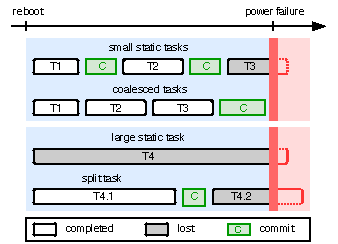
\includegraphics[width=\columnwidth]{figures/intro-figure-vert.pdf}
    \caption{Task coalescing at runtime reduces time and energy overhead in task-based intermittent programming models by performing fewer commits (denoted as \texttt{cmt} in the figure). On the other hand, task splitting reduces wasted computation and enables termination for bigger tasks.}
    \label{fig:coalesce}
\end{figure}

\textbf{Task Decomposition of Intermittent Programs.} {\em
Task-based} programming and execution models require a
programmer~\cite{alpaca,chain} or a compiler~\cite{baghsorkhi_cgo_2018} to
statically decompose a program into a collection of {\em tasks}.  A task can
include arbitrary computation that should be executed despite arbitrarily-timed power failures.
%and these existing systems guarantee that each
%tasks executes {\em atomically}, despite arbitrarily-timed power failures.
%
The programmer (or a compiler) explicitly expresses task-to-task control flow.
%
Figure~\ref{fig:coalesce} illustrates how a program's tasks execute and
shows how tasks can impose a run-time overhead. At each task transition, the system incurs an overhead to track and atomically \emph{commit} modifications to the non-volatile memory, to maintain consistency of program state~\cite{chain,alpaca}. The more task transitions a program requires, the more commit overhead is incurred by the system at run-time.

A programmer may thus create very large tasks in an attempt to reduce
overhead by minimizing the number of task transitions. However, a very large
task may require more energy to complete than a device's fixed hardware energy
buffer can hold which may lead to a program non-termination problem. To eliminate this risk,
existing systems require the programmer to decompose a program
into small tasks, all of which complete using only buffered energy. These
constraints on task sizing leave an unsatisfying dilemma: large, efficient
tasks that risk non-termination, or small tasks that are guaranteed to
complete, but incur a high task transition and commit overhead. In this work,
we propose a third way, using a novel technique called {\em adaptive execution by dynamic task
coalescing/splitting} that efficiently executes small tasks, trimming unnecessary overheads, while avoiding the risk of non-termination.

%A key challenge is that the length of a software
%task's execution is \emph{limited by the fixed total amount of energy} that a
%device can buffer in hardware. A task's code is static, but the duration of its
%execution may be input-dependent and is difficult to predict. To illustrate
%this, we refer to Figure~\ref{fig:1} showing the execution time of two
%applications (the same application X, but divided into X and Y tasks as
%in~\cite{chain}) running on RFID antenna-powered Computational
%RFID~\cite{wisp,rf_powered_computing_gollakota_2014} at two device-to-antenna
%distances (near---stable energy supply/far---high energy intermittency). At
%short distance: execution will takes too long caused by runtime cost of
%marshalling excessively small tasks. At far distance: program \emph{might never
%execute} if task execution consumes more energy than the system can buffer.
%This calls for at-runtime adaptive task division of any transiently-powered
%application---namely \emph{task virtualization}.

This paper introduces a new system called \sys, which executes a task-based
intermittent program by dynamically coalescing/splitting its tasks.
\sys accepts any static decomposition and coalesces/splits its tasks at runtime. Two consecutive, coalesced tasks execute
with no commit overhead between them, instead performing
task-end commit actions at the end of the second task only.
%
When there is sufficient energy to execute both tasks, two distinct, small
tasks are effectively executed as a single large task, preserving the atomicity
of both. If power fails during a coalesced task, execution restarts from the
{\em first} of the coalesced tasks. Figure~\ref{fig:coalesce} (top)
illustrates how dynamic coalescing removes unnecessary overhead and shortens intermittent program execution.
On the other hand, a large task that requires more energy to complete than a device buffered energy
is split by \sys to enable task termination and preserve execution progress, as depicted in Figure~\ref{fig:coalesce} (bottom).

%Brandon: This is too detailed for the intro:
%Unfortunately, naively merging two atomic tasks might produce a non-atomic
%task, that may leave non-volatile memory inconsistent after a partial
%execution. A merge breaks atomicity when atomic merged tasks form a
%\emph{write-after-read (WAR)} dependency---for instance if two tasks
%\texttt{\{x=y+1\}; \{y=x;\}} are merged and if the power failure occurs after
%\texttt{x=y}, the value \texttt{x} will be increased twice when the merged task
%is restarted, that leads to an inconsistency.

%variables in non-volatile memory at \emph{run-time} that can
%break the atomicity of the \emph{virtual task}. Consider the
%example depicted in Fig.~\ref{fig:virtualization}: Tasks 1,
%2 and 3 being executed consecutively. All tasks in this
%example are atomic since they do not have WAR dependency on
%the persistent variables they are accessing, e.g. \emph{x}
%is only read and \emph{y} is only written within Task 1.
%Now, suppose three tasks have been virtualized into a single
%one at run-time, namely Task 4: since \emph{x} is now first
%\emph{read} and then \emph{written}, a WAR dependency on
%\emph{x} is introduced dynamically at
%run-time---unfortunately Task 4 is \emph{no more atomic}
%since its re-execution will not always produce the same
%results.
\textbf{Challenges and Contributions} 
\begin{itemize}
\item\textit{challenge} 1) Given unpredictable energy shots arrival, how to specify the size of a dynamic task on the fly? \textit{contribution---1} \sys addresses this challenge by using its \textit{recent execution history} as a metric to estimate the environment energy conditions. Furthermore, It mitigates the risk of dynamic task re-execution by taking advantage of the certainty that the energy buffer offers and approaches the expected power interrupt carefully. 
%
\item\textit{challenge} 2) Given dynamic variables dependencies, how to ensure efficient data protection against power interrupts? \textit{contribution---2} \sys ensures the consistency of the data by using a novel
approach called \emph{dynamic group privatization}. Varying variables dependencies forces a static approach (i.e.~\cite{alpaca}) to operate by considering a worst case scenario (i.e. protecting all global variables) in each dynamic task transition. \sys, therefore, utilizes a real-time data tracking to enable partial data protection on a task transition. Individual variables tacking, however, slows down a system dramatically. Therefore, \sys  relies on a coarse locality principle and protects the global variables in a batch. Moreover, it optimizes the data transfer by using Direct Memory Access (DMA).

\item\textit{challenge} 3) A static task decomposition model assumes that each
single task can execute to completion. If the hardware energy buffer provides
inadequate energy to execute each single task to completion, a program will not
terminate~\cite{cleancut_2018}. under such conditions how to enable the dynamic execution model to progress on a sub-task level? \textit{contribution---3} To avoid non-termination under adversarial
energy conditions, \sys uses a timer-based {\em partial task commit} mechanism.
Partial execution avoids non-termination by committing the intermediate state of a long-running
task that has repeatedly failed and restarted. Partial execution violates
task atomicity, but preserves forward progress; if a programmer knows that
task atomicity is crucial to correctness, they can disable partial execution around a piece of code.

% \textbf{dynamic privatization}: while a compiler can use static data privatization and commit instrumentation
% (i.e., redo-logging) to eliminate statically identifiable, inter-task data
% dependences~\cite{alpaca}, a \emph{dynamic} dependence between two coalesced
% tasks requires dynamic privatization and commit actions.
% %

%
%Therefore, we require a \emph{new execution
%model} that keeps each virtual task atomic by committing the
%modified persistent variables at the boundary defined
%dynamically at run-time---keeping the non-volatile memory
%unmodified upon a power-interrupt and preserving its
%consistency.
% \textbf{task non-termination}: 

%
% !!!! % It should be emphasized that unlike a voltage-threshold-based protection approaches that may suffer from a non-termination problem if the checkpoint has to be placed within the interrupt-disabled region, a timer-based approach adapts its partial commit location on repeated failures.
%
%Task coalescing removes the burden from the programmer, because it accepts any
%task decomposition and improves it dynamically. To further reduce the
%programmer effort, we propose a compiler pass for \emph{automatic
%decomposition} of programs into (small) \emph{atomic} tasks. The compiler
%identifies non-volatile variables shared across tasks as tasks are created, and
%instruments reads and writes of those variables, using memory virtualization,
%to keep the data consistent in the presence of power loss.
%
%\textcolor{red}{Despite being limited to a subset of the C language, the
%automatic task decomposition allowed us to port several	applications to an
%intermittent platform with a moderate effort.}
%
\end{itemize}

% \textbf{Contributions.} To summarize, \sys's main contributions are:
% %
% \begin{itemize}
% \item The first {\em adaptive} task-based intermittent execution model that
% dynamically \emph{coalesces} tasks to reduce commit overhead and
% \emph{downscales} tasks to ensure forward progress.
% \item The first memory virtualization mechanism that preserves the atomicity of coalesced tasks under power failures.
% %\item A fall-back dynamic task splitting mechanism that preserves forward progress despite executing tasks that are too large for a device's energy supply.
% \item A fully-realized prototype of \sys that runs on real energy-harvesting devices, to be released as open source after publication via~\cite{coala_website}.
% \item An evaluation directly comparing \sys to a state of the art task-based
% intermittent programming and execution model from prior work, showing that on a
% suite of benchmarks from the literature and several new workloads, \sys often
% has higher performance and is more flexible to diverse energy conditions.
% \end{itemize}
%
Section~\ref{sec:background} provides background on intermittent computing.
Section~\ref{sec:systemdescription} provides an overview of \sys, while
Section~\ref{sec:task_adaptation} describes \sys's task adaptation mechanism (coalescing and downscaling). Memory virtualization mechanism is provided in Section~\ref{sec:memory_virtulaization}. Implementation details of \sys are given in Section~\ref{sec:implementation}. Sections~\ref{sec:methodology} and~\ref{sec:evaluation} describe \sys's methodology and evaluation, respectively. Section~\ref{sec:related_work} puts \sys in the
context of related work and Section~\ref{sec:conclusions} concludes and discusses
future work.

